\section{Description}
The purpose of this project is to take the well-known Particle Swarm Optimization \cite{Blondin2009} and hardware acceleration calculations on the Zybo xc7z010clg-400-1 board. By using this board and the accompanying Xilinx tools the algorithm will be split into parts that run in software and others in hardware. 
\\\\
As seen in the rich picture on figure \ref{fig:descriptiondiagram}. A researcher often sits in his or her lab solving problems of mathematical nature. The projects varies from groundbreaking university research to helping the industry partners solve problems. An ongoing theme is the need to find a objective function hence the desire to maximize or minimize.
The researcher's preferred tool is particle swarm optimization because it can find the global maximum or minimum, but the drawback is that it takes a long time to calculate on the devices they have available. Therefore using a new Zybo xc7z010clg-400-1 board where the critical parts of the algorithm will be hardware accelerated. Using this solution they can save time that would be better spent elsewhere.

\begin{figure}[!h]
	\centering
	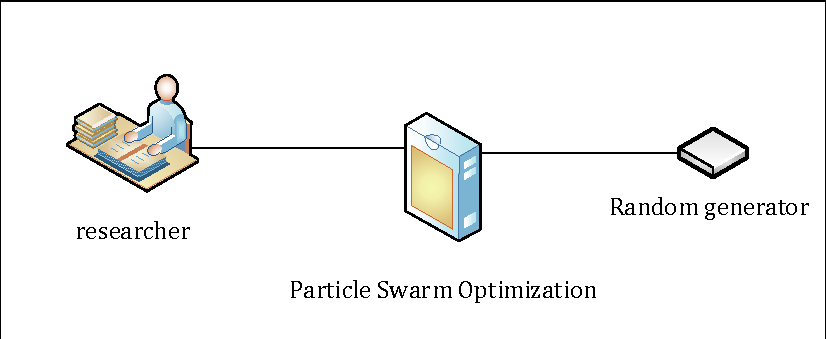
\includegraphics[width=0.7\linewidth]{diagram/description_diagram}
	\caption{Researcher who is using the Particle Swarm Optimization System and a audio source to generate the random element }
	\label{fig:descriptiondiagram}
\end{figure}